\begin{BPMN}{PROC-03}{Revisar Plan de Estudios y mapa curricular}{}
    \PCitem{Participantes}{Jefe de desarrollo e innovación curricular y Analista de la DES}
    \PCitem{Objetivo}{Revisar la documentación enviada por la Unidad Académica con respecto al Plan de Estudios y mapa curricular a fin de determinar si es aprobado o se regresa a correcciones}
    \PCitem{Interrelación con otros procesos }{Elaboración de Plan de Estudios y Creacion de Unidad de Aprendizaje }
    \PCitem{Proveedores}{Unidad Académica(Subdirector, Jefe de innovación educativa y docentes)}
    \PCitem{Entradas}{Documento de Plan de Estudios y Mapa curricular}
    \PCitem{Consumidores}{Unidad Académica}
    \PCitem{Salidas}{Dictamen de Aprobación de Plan de Estudios }
    \PCitem{Precondiciones}{Elaboración y envió del Plan de Estudios y Mapa curricular}
    \PCitem{PostCondiciones}{Envio del oficio de aprobación del Plan de estudios o Envio del Plan de Estudios con notas}
    \PCitem{Frecuencia}{}
    \PCitem{Tipo}{Soporte}
    \PCitem {Áreas de oportunidad}{Intercambio de los documentos, asignación de personal a tareas y generación de notas}
\end{BPMN}
En la figura \hyperref[]{}
\begin{figure}[htbp]
	\begin{center}
		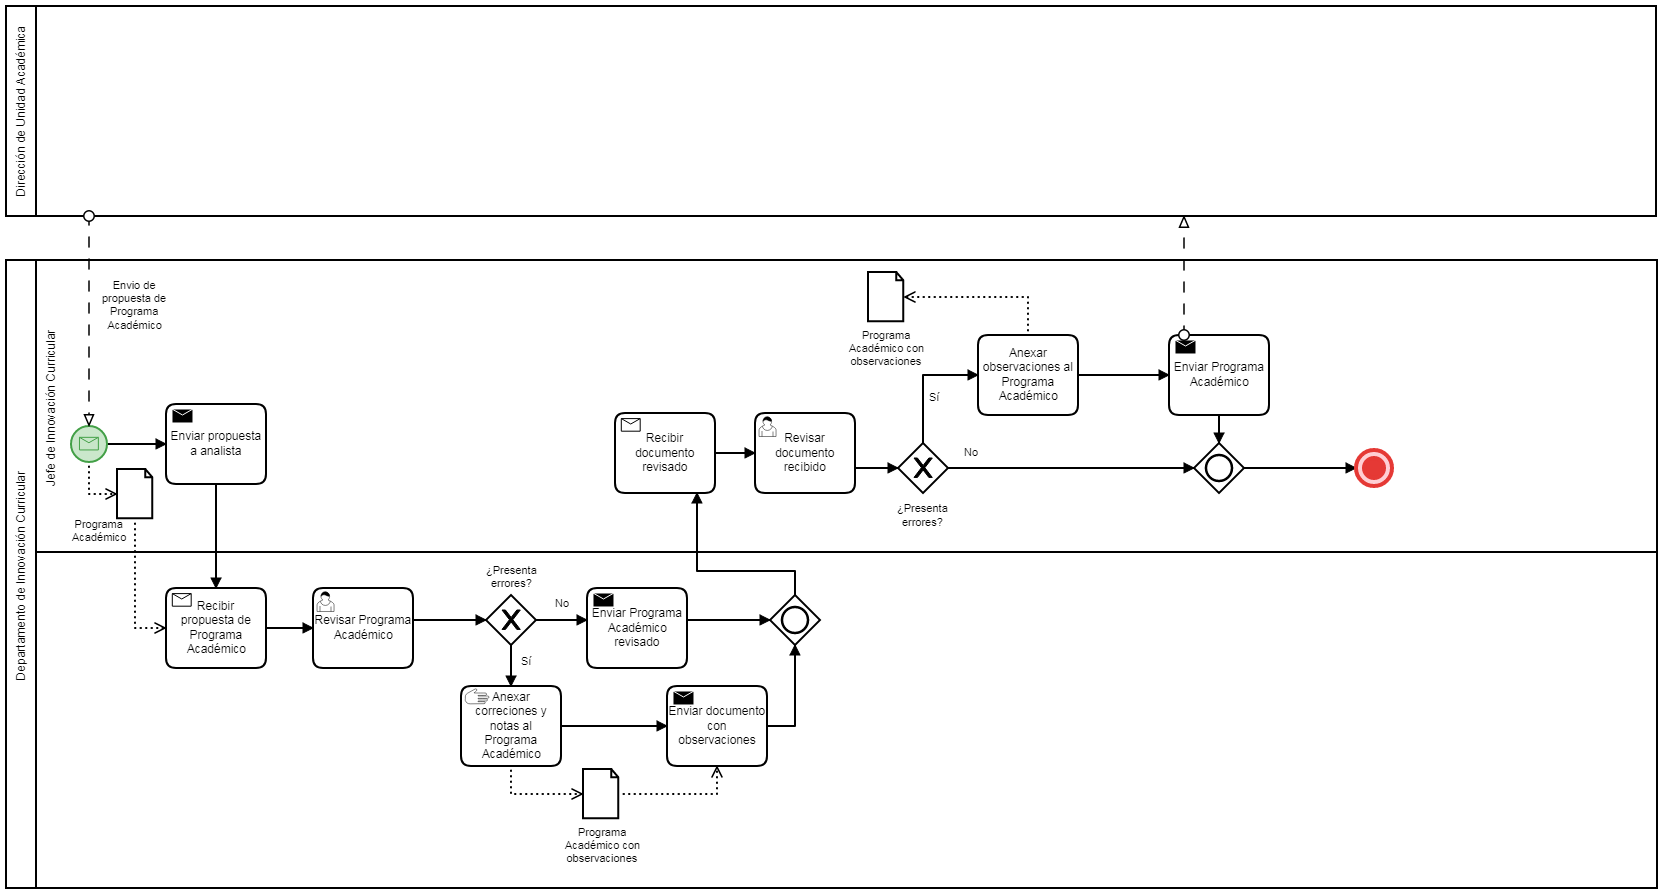
\includegraphics[width=.95\textwidth]{C1-DP/SP5/proceso_validarPA.png}
		\caption{}
		\label{fig:}
	\end{center}
\end{figure}